\section{Spark::Sp\-Vertex\-Noise\-Sb Class Reference}
\label{classSpark_1_1SpVertexNoiseSb}\index{Spark::SpVertexNoiseSb@{Spark::SpVertexNoiseSb}}
{\tt \#include $<$Sp\-Vertex\-Noise\-Sb.h$>$}

Inheritance diagram for Spark::Sp\-Vertex\-Noise\-Sb:\begin{figure}[H]
\begin{center}
\leavevmode
\includegraphics[width=82pt]{classSpark_1_1SpVertexNoiseSb__inherit__graph}
\end{center}
\end{figure}
Collaboration diagram for Spark::Sp\-Vertex\-Noise\-Sb:\begin{figure}[H]
\begin{center}
\leavevmode
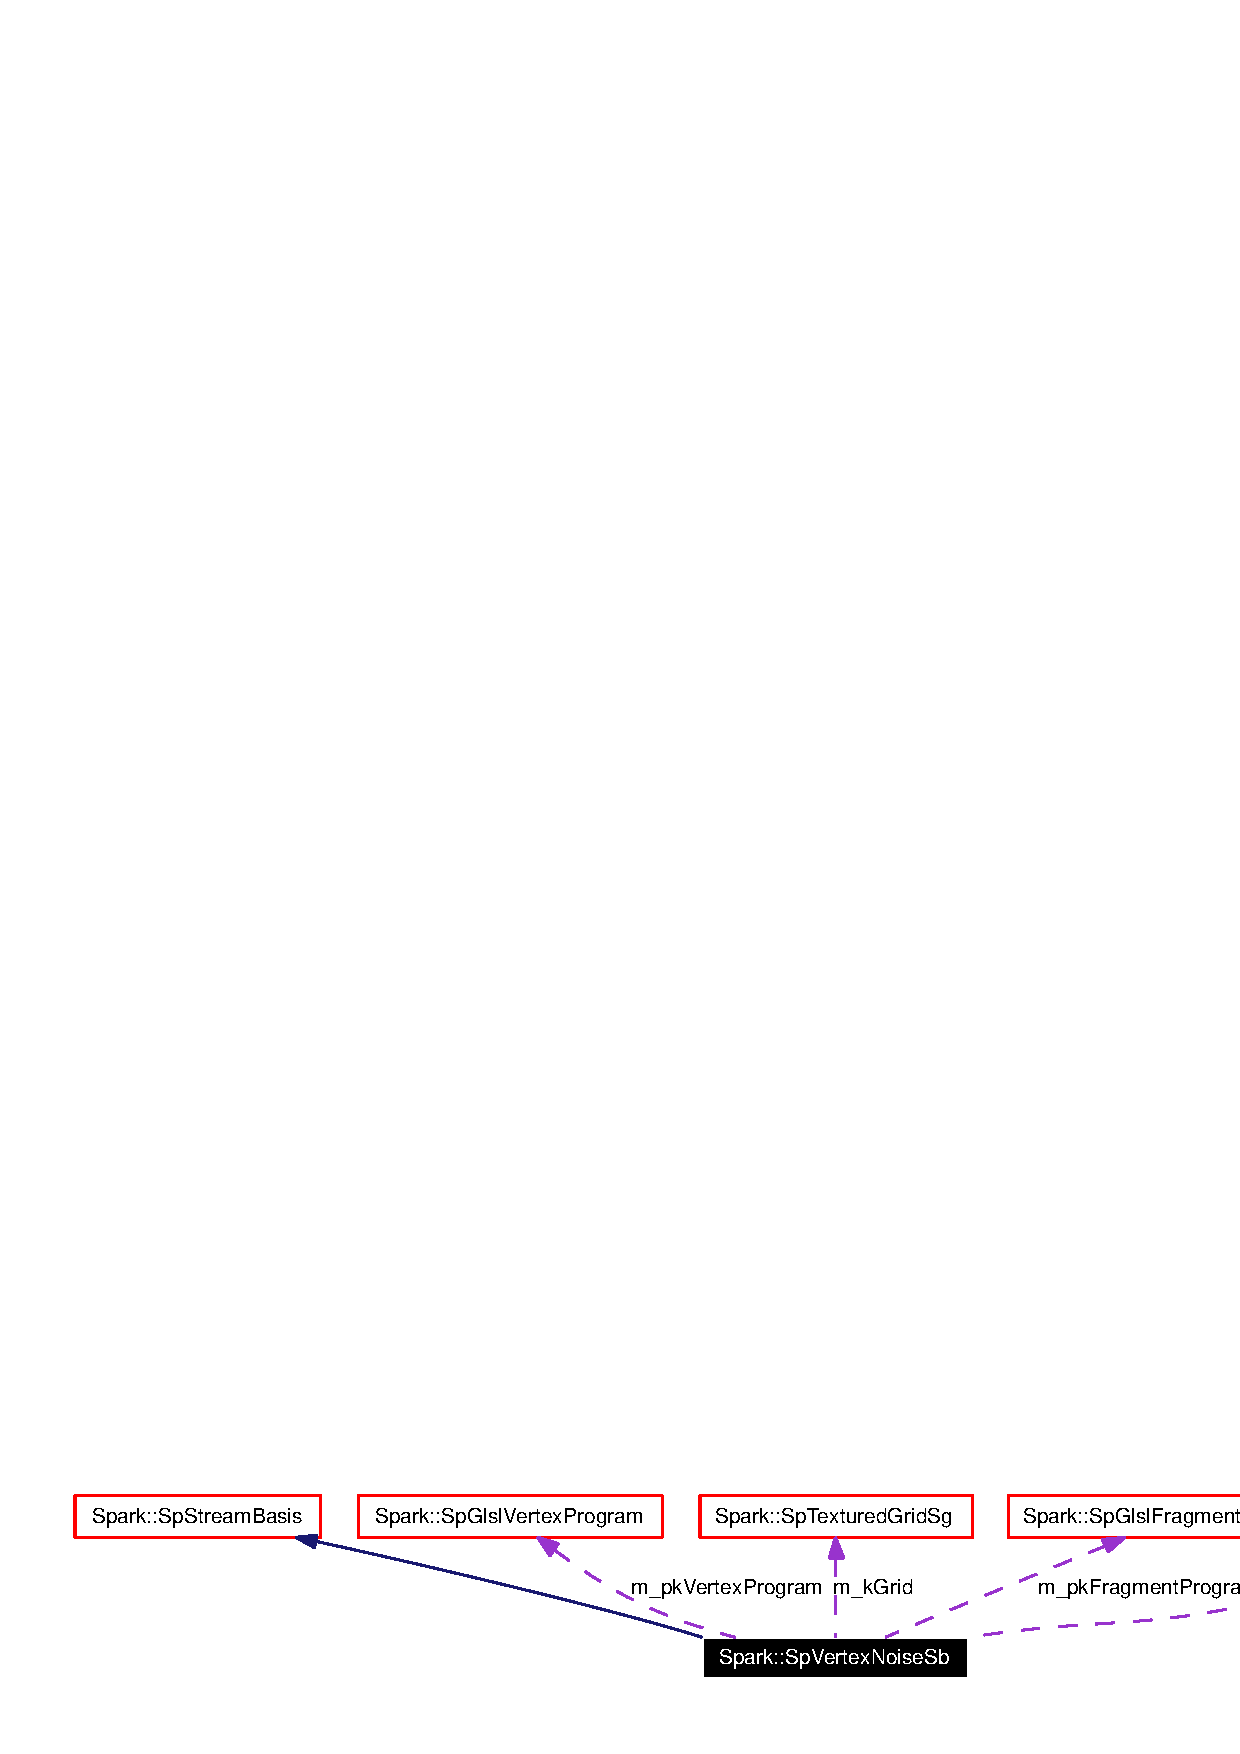
\includegraphics[width=395pt]{classSpark_1_1SpVertexNoiseSb__coll__graph}
\end{center}
\end{figure}


\subsection{Detailed Description}
Noise generating stream basis which operates on vertex data. 

Definition at line 40 of file Sp\-Vertex\-Noise\-Sb.h.\subsection*{Public Member Functions}
\begin{CompactItemize}
\item 
{\bf Sp\-Vertex\-Noise\-Sb} (bool b\-Abs\-Noise=false, float f\-Offset\-X=1, float f\-Offset\-Y=1, float f\-Offset\-Z=1, float f\-Scale\-X=1, float f\-Scale\-Y=1, float f\-Scale\-Z=1, unsigned int ui\-Grid\-Resolution=150, unsigned long i\-Seed=1234)
\begin{CompactList}\small\item\em Construction:. \item\end{CompactList}\item 
virtual {\bf $\sim$Sp\-Vertex\-Noise\-Sb} ()
\item 
void {\bf initialize} ()
\begin{CompactList}\small\item\em Operations:. \item\end{CompactList}\item 
void {\bf destroy} ()
\item 
void {\bf preload} ()
\item 
void {\bf enable} ()
\item 
void {\bf disable} ()
\item 
virtual void {\bf set\-Scale} (float f\-X, float f\-Y, float f\-Z)
\item 
virtual void {\bf get\-Scale} (float \&rf\-X, float \&rf\-Y, float \&rf\-Z) const
\item 
virtual void {\bf set\-Offset} (float f\-X, float f\-Y, float f\-Z)
\item 
virtual void {\bf get\-Offset} (float \&rf\-X, float \&rf\-Y, float \&rf\-Z) const
\item 
virtual void {\bf set\-Weight} (float f\-Weight)
\item 
virtual float {\bf get\-Weight} () const
\item 
void {\bf set\-Grid\-Resolution} (unsigned int ui\-Resolution)
\item 
{\bf Sp\-Glsl\-Vertex\-Program} $\ast$ {\bf program} ()
\item 
virtual bool {\bf has\-Changed} ()
\begin{CompactList}\small\item\em Inherited Methods:. \item\end{CompactList}\item 
virtual bool {\bf send\-Output\-To\-Buffer} ({\bf Sp\-Stream\-Buffer} $\ast$pk\-Buffer, {\bf Sp\-Copy\-To\-Texture\-Fb} $\ast$pk\-Copy)
\end{CompactItemize}
\subsection*{Protected Attributes}
\begin{CompactItemize}
\item 
{\bf Sp\-Glsl\-Vertex\-Program} $\ast$ {\bf m\_\-pk\-Vertex\-Program}
\begin{CompactList}\small\item\em Internal Data:. \item\end{CompactList}\item 
{\bf Sp\-Glsl\-Fragment\-Program} $\ast$ {\bf m\_\-pk\-Fragment\-Program}
\item 
int $\ast$ {\bf m\_\-ai\-P}
\item 
{\bf Sp\-Vector4f} $\ast$ {\bf m\_\-ak\-PG}
\item 
bool {\bf m\_\-b\-Is\-Initialized}
\item 
bool {\bf m\_\-b\-Has\-Changed}
\item 
unsigned long {\bf m\_\-ul\-Seed}
\item 
{\bf Sp\-Textured\-Grid\-Sg} {\bf m\_\-k\-Grid}
\item 
float {\bf m\_\-f\-Offset\-X}
\item 
float {\bf m\_\-f\-Offset\-Y}
\item 
float {\bf m\_\-f\-Offset\-Z}
\item 
float {\bf m\_\-f\-Scale\-X}
\item 
float {\bf m\_\-f\-Scale\-Y}
\item 
float {\bf m\_\-f\-Scale\-Z}
\item 
float {\bf m\_\-f\-Weight}
\end{CompactItemize}


\subsection{Constructor \& Destructor Documentation}
\index{Spark::SpVertexNoiseSb@{Spark::Sp\-Vertex\-Noise\-Sb}!SpVertexNoiseSb@{SpVertexNoiseSb}}
\index{SpVertexNoiseSb@{SpVertexNoiseSb}!Spark::SpVertexNoiseSb@{Spark::Sp\-Vertex\-Noise\-Sb}}
\subsubsection{\setlength{\rightskip}{0pt plus 5cm}Sp\-Vertex\-Noise\-Sb::Sp\-Vertex\-Noise\-Sb (bool {\em b\-Abs\-Noise} = {\tt false}, float {\em f\-Offset\-X} = {\tt 1}, float {\em f\-Offset\-Y} = {\tt 1}, float {\em f\-Offset\-Z} = {\tt 1}, float {\em f\-Scale\-X} = {\tt 1}, float {\em f\-Scale\-Y} = {\tt 1}, float {\em f\-Scale\-Z} = {\tt 1}, unsigned int {\em ui\-Grid\-Resolution} = {\tt 150}, unsigned long {\em i\-Seed} = {\tt 1234})}\label{classSpark_1_1SpVertexNoiseSb_a0}


Construction:. 

Definition at line 23 of file Sp\-Vertex\-Noise\-Sb.cpp.

References Spark::Sp\-Glsl\-Manager::load\-Fragment\-Program\-From\-File(), Spark::Sp\-Glsl\-Manager::load\-Vertex\-Program\-From\-File(), m\_\-b\-Has\-Changed, m\_\-k\-Grid, m\_\-pk\-Fragment\-Program, m\_\-pk\-Vertex\-Program, and Spark::Sp\-Textured\-Grid\-Sg::set\-Resolution().\index{Spark::SpVertexNoiseSb@{Spark::Sp\-Vertex\-Noise\-Sb}!~SpVertexNoiseSb@{$\sim$SpVertexNoiseSb}}
\index{~SpVertexNoiseSb@{$\sim$SpVertexNoiseSb}!Spark::SpVertexNoiseSb@{Spark::Sp\-Vertex\-Noise\-Sb}}
\subsubsection{\setlength{\rightskip}{0pt plus 5cm}Sp\-Vertex\-Noise\-Sb::$\sim${\bf Sp\-Vertex\-Noise\-Sb} ()\hspace{0.3cm}{\tt  [virtual]}}\label{classSpark_1_1SpVertexNoiseSb_a1}


Definition at line 64 of file Sp\-Vertex\-Noise\-Sb.cpp.

References destroy().

\subsection{Member Function Documentation}
\index{Spark::SpVertexNoiseSb@{Spark::Sp\-Vertex\-Noise\-Sb}!destroy@{destroy}}
\index{destroy@{destroy}!Spark::SpVertexNoiseSb@{Spark::Sp\-Vertex\-Noise\-Sb}}
\subsubsection{\setlength{\rightskip}{0pt plus 5cm}void Sp\-Vertex\-Noise\-Sb::destroy ()}\label{classSpark_1_1SpVertexNoiseSb_a3}


Definition at line 132 of file Sp\-Vertex\-Noise\-Sb.cpp.

References m\_\-ai\-P, m\_\-ak\-PG, m\_\-pk\-Vertex\-Program, and Spark::Sp\-Glsl\-Manager::release().

Referenced by $\sim$Sp\-Vertex\-Noise\-Sb().\index{Spark::SpVertexNoiseSb@{Spark::Sp\-Vertex\-Noise\-Sb}!disable@{disable}}
\index{disable@{disable}!Spark::SpVertexNoiseSb@{Spark::Sp\-Vertex\-Noise\-Sb}}
\subsubsection{\setlength{\rightskip}{0pt plus 5cm}void Sp\-Vertex\-Noise\-Sb::disable ()}\label{classSpark_1_1SpVertexNoiseSb_a6}


Definition at line 172 of file Sp\-Vertex\-Noise\-Sb.cpp.

References Spark::Sp\-Glsl\-Manager::disable(), m\_\-pk\-Fragment\-Program, and m\_\-pk\-Vertex\-Program.

Referenced by send\-Output\-To\-Buffer().\index{Spark::SpVertexNoiseSb@{Spark::Sp\-Vertex\-Noise\-Sb}!enable@{enable}}
\index{enable@{enable}!Spark::SpVertexNoiseSb@{Spark::Sp\-Vertex\-Noise\-Sb}}
\subsubsection{\setlength{\rightskip}{0pt plus 5cm}void Sp\-Vertex\-Noise\-Sb::enable ()}\label{classSpark_1_1SpVertexNoiseSb_a5}


Definition at line 154 of file Sp\-Vertex\-Noise\-Sb.cpp.

References Spark::Sp\-Glsl\-Manager::enable(), initialize(), m\_\-b\-Is\-Initialized, m\_\-f\-Weight, m\_\-pk\-Fragment\-Program, m\_\-pk\-Vertex\-Program, and Spark::Sp\-Glsl\-Vertex\-Program::set\-Parameter1f().

Referenced by send\-Output\-To\-Buffer().\index{Spark::SpVertexNoiseSb@{Spark::Sp\-Vertex\-Noise\-Sb}!getOffset@{getOffset}}
\index{getOffset@{getOffset}!Spark::SpVertexNoiseSb@{Spark::Sp\-Vertex\-Noise\-Sb}}
\subsubsection{\setlength{\rightskip}{0pt plus 5cm}virtual void Spark::Sp\-Vertex\-Noise\-Sb::get\-Offset (float \& {\em rf\-X}, float \& {\em rf\-Y}, float \& {\em rf\-Z}) const\hspace{0.3cm}{\tt  [inline, virtual]}}\label{classSpark_1_1SpVertexNoiseSb_a10}




Reimplemented from {\bf Spark::Sp\-Stream\-Basis} {\rm (p.\,\pageref{classSpark_1_1SpStreamBasis_a7})}.

Definition at line 87 of file Sp\-Vertex\-Noise\-Sb.h.

References m\_\-f\-Offset\-X, m\_\-f\-Offset\-Y, and m\_\-f\-Offset\-Z.\index{Spark::SpVertexNoiseSb@{Spark::Sp\-Vertex\-Noise\-Sb}!getScale@{getScale}}
\index{getScale@{getScale}!Spark::SpVertexNoiseSb@{Spark::Sp\-Vertex\-Noise\-Sb}}
\subsubsection{\setlength{\rightskip}{0pt plus 5cm}virtual void Spark::Sp\-Vertex\-Noise\-Sb::get\-Scale (float \& {\em rf\-X}, float \& {\em rf\-Y}, float \& {\em rf\-Z}) const\hspace{0.3cm}{\tt  [inline, virtual]}}\label{classSpark_1_1SpVertexNoiseSb_a8}




Reimplemented from {\bf Spark::Sp\-Stream\-Basis} {\rm (p.\,\pageref{classSpark_1_1SpStreamBasis_a9})}.

Definition at line 72 of file Sp\-Vertex\-Noise\-Sb.h.

References m\_\-f\-Scale\-X, m\_\-f\-Scale\-Y, and m\_\-f\-Scale\-Z.\index{Spark::SpVertexNoiseSb@{Spark::Sp\-Vertex\-Noise\-Sb}!getWeight@{getWeight}}
\index{getWeight@{getWeight}!Spark::SpVertexNoiseSb@{Spark::Sp\-Vertex\-Noise\-Sb}}
\subsubsection{\setlength{\rightskip}{0pt plus 5cm}virtual float Spark::Sp\-Vertex\-Noise\-Sb::get\-Weight () const\hspace{0.3cm}{\tt  [inline, virtual]}}\label{classSpark_1_1SpVertexNoiseSb_a12}


Definition at line 100 of file Sp\-Vertex\-Noise\-Sb.h.

References m\_\-f\-Weight.\index{Spark::SpVertexNoiseSb@{Spark::Sp\-Vertex\-Noise\-Sb}!hasChanged@{hasChanged}}
\index{hasChanged@{hasChanged}!Spark::SpVertexNoiseSb@{Spark::Sp\-Vertex\-Noise\-Sb}}
\subsubsection{\setlength{\rightskip}{0pt plus 5cm}bool Sp\-Vertex\-Noise\-Sb::has\-Changed ()\hspace{0.3cm}{\tt  [virtual]}}\label{classSpark_1_1SpVertexNoiseSb_a15}


Inherited Methods:. 



Implements {\bf Spark::Sp\-Stream\-Basis} {\rm (p.\,\pageref{classSpark_1_1SpStreamBasis_a2})}.

Definition at line 182 of file Sp\-Vertex\-Noise\-Sb.cpp.

References m\_\-b\-Has\-Changed.\index{Spark::SpVertexNoiseSb@{Spark::Sp\-Vertex\-Noise\-Sb}!initialize@{initialize}}
\index{initialize@{initialize}!Spark::SpVertexNoiseSb@{Spark::Sp\-Vertex\-Noise\-Sb}}
\subsubsection{\setlength{\rightskip}{0pt plus 5cm}void Sp\-Vertex\-Noise\-Sb::initialize ()}\label{classSpark_1_1SpVertexNoiseSb_a2}


Operations:. 

Definition at line 69 of file Sp\-Vertex\-Noise\-Sb.cpp.

References Spark::Sp\-Glsl\-Manager::bind(), Spark::Sp\-Glsl\-Manager::compile(), m\_\-ai\-P, m\_\-ak\-PG, m\_\-b\-Is\-Initialized, m\_\-pk\-Vertex\-Program, m\_\-ul\-Seed, Spark::Normalize(), Spark::Random\-Symmetric\-Float(), Spark::Random\-UInt(), Spark::Seed\-Random(), Spark::Sp\-Glsl\-Vertex\-Program::set\-Parameter4fv(), and Spark::Sp\-Vector4f.

Referenced by enable(), and preload().\index{Spark::SpVertexNoiseSb@{Spark::Sp\-Vertex\-Noise\-Sb}!preload@{preload}}
\index{preload@{preload}!Spark::SpVertexNoiseSb@{Spark::Sp\-Vertex\-Noise\-Sb}}
\subsubsection{\setlength{\rightskip}{0pt plus 5cm}void Sp\-Vertex\-Noise\-Sb::preload ()}\label{classSpark_1_1SpVertexNoiseSb_a4}


Definition at line 148 of file Sp\-Vertex\-Noise\-Sb.cpp.

References initialize(), and m\_\-b\-Is\-Initialized.\index{Spark::SpVertexNoiseSb@{Spark::Sp\-Vertex\-Noise\-Sb}!program@{program}}
\index{program@{program}!Spark::SpVertexNoiseSb@{Spark::Sp\-Vertex\-Noise\-Sb}}
\subsubsection{\setlength{\rightskip}{0pt plus 5cm}{\bf Sp\-Glsl\-Vertex\-Program}$\ast$ Spark::Sp\-Vertex\-Noise\-Sb::program ()\hspace{0.3cm}{\tt  [inline]}}\label{classSpark_1_1SpVertexNoiseSb_a14}


Definition at line 111 of file Sp\-Vertex\-Noise\-Sb.h.

References m\_\-pk\-Vertex\-Program.\index{Spark::SpVertexNoiseSb@{Spark::Sp\-Vertex\-Noise\-Sb}!sendOutputToBuffer@{sendOutputToBuffer}}
\index{sendOutputToBuffer@{sendOutputToBuffer}!Spark::SpVertexNoiseSb@{Spark::Sp\-Vertex\-Noise\-Sb}}
\subsubsection{\setlength{\rightskip}{0pt plus 5cm}bool Sp\-Vertex\-Noise\-Sb::send\-Output\-To\-Buffer ({\bf Sp\-Stream\-Buffer} $\ast$ {\em pk\-Buffer}, {\bf Sp\-Copy\-To\-Texture\-Fb} $\ast$ {\em pk\-Copy})\hspace{0.3cm}{\tt  [virtual]}}\label{classSpark_1_1SpVertexNoiseSb_a16}


Definition at line 187 of file Sp\-Vertex\-Noise\-Sb.cpp.

References Spark::Sp\-Stream\-Buffer::disable(), disable(), enable(), Spark::Sp\-Stream\-Buffer::enable(), Spark::Sp\-Stream\-Buffer::is\-Double\-Buffered(), Spark::Sp\-Stream\-Buffer::is\-Initialized(), m\_\-b\-Has\-Changed, m\_\-f\-Offset\-X, m\_\-f\-Offset\-Y, m\_\-f\-Offset\-Z, m\_\-f\-Scale\-X, m\_\-f\-Scale\-Y, m\_\-f\-Scale\-Z, m\_\-k\-Grid, Spark::Sp\-Textured\-Grid\-Sg::render(), and Spark::Sp\-Copy\-To\-Texture\-Fb::update\-Output().\index{Spark::SpVertexNoiseSb@{Spark::Sp\-Vertex\-Noise\-Sb}!setGridResolution@{setGridResolution}}
\index{setGridResolution@{setGridResolution}!Spark::SpVertexNoiseSb@{Spark::Sp\-Vertex\-Noise\-Sb}}
\subsubsection{\setlength{\rightskip}{0pt plus 5cm}void Spark::Sp\-Vertex\-Noise\-Sb::set\-Grid\-Resolution (unsigned int {\em ui\-Resolution})\hspace{0.3cm}{\tt  [inline]}}\label{classSpark_1_1SpVertexNoiseSb_a13}


Definition at line 105 of file Sp\-Vertex\-Noise\-Sb.h.

References m\_\-b\-Has\-Changed, m\_\-k\-Grid, and Spark::Sp\-Textured\-Grid\-Sg::set\-Resolution().\index{Spark::SpVertexNoiseSb@{Spark::Sp\-Vertex\-Noise\-Sb}!setOffset@{setOffset}}
\index{setOffset@{setOffset}!Spark::SpVertexNoiseSb@{Spark::Sp\-Vertex\-Noise\-Sb}}
\subsubsection{\setlength{\rightskip}{0pt plus 5cm}virtual void Spark::Sp\-Vertex\-Noise\-Sb::set\-Offset (float {\em f\-X}, float {\em f\-Y}, float {\em f\-Z})\hspace{0.3cm}{\tt  [inline, virtual]}}\label{classSpark_1_1SpVertexNoiseSb_a9}




Reimplemented from {\bf Spark::Sp\-Stream\-Basis} {\rm (p.\,\pageref{classSpark_1_1SpStreamBasis_a6})}.

Definition at line 79 of file Sp\-Vertex\-Noise\-Sb.h.

References m\_\-b\-Has\-Changed, m\_\-f\-Offset\-X, m\_\-f\-Offset\-Y, and m\_\-f\-Offset\-Z.\index{Spark::SpVertexNoiseSb@{Spark::Sp\-Vertex\-Noise\-Sb}!setScale@{setScale}}
\index{setScale@{setScale}!Spark::SpVertexNoiseSb@{Spark::Sp\-Vertex\-Noise\-Sb}}
\subsubsection{\setlength{\rightskip}{0pt plus 5cm}virtual void Spark::Sp\-Vertex\-Noise\-Sb::set\-Scale (float {\em f\-X}, float {\em f\-Y}, float {\em f\-Z})\hspace{0.3cm}{\tt  [inline, virtual]}}\label{classSpark_1_1SpVertexNoiseSb_a7}




Reimplemented from {\bf Spark::Sp\-Stream\-Basis} {\rm (p.\,\pageref{classSpark_1_1SpStreamBasis_a8})}.

Definition at line 64 of file Sp\-Vertex\-Noise\-Sb.h.

References m\_\-b\-Has\-Changed, m\_\-f\-Scale\-X, m\_\-f\-Scale\-Y, and m\_\-f\-Scale\-Z.\index{Spark::SpVertexNoiseSb@{Spark::Sp\-Vertex\-Noise\-Sb}!setWeight@{setWeight}}
\index{setWeight@{setWeight}!Spark::SpVertexNoiseSb@{Spark::Sp\-Vertex\-Noise\-Sb}}
\subsubsection{\setlength{\rightskip}{0pt plus 5cm}virtual void Spark::Sp\-Vertex\-Noise\-Sb::set\-Weight (float {\em f\-Weight})\hspace{0.3cm}{\tt  [inline, virtual]}}\label{classSpark_1_1SpVertexNoiseSb_a11}




Reimplemented from {\bf Spark::Sp\-Stream\-Basis} {\rm (p.\,\pageref{classSpark_1_1SpStreamBasis_a4})}.

Definition at line 94 of file Sp\-Vertex\-Noise\-Sb.h.

References m\_\-b\-Has\-Changed, and m\_\-f\-Weight.

\subsection{Member Data Documentation}
\index{Spark::SpVertexNoiseSb@{Spark::Sp\-Vertex\-Noise\-Sb}!m_aiP@{m\_\-aiP}}
\index{m_aiP@{m\_\-aiP}!Spark::SpVertexNoiseSb@{Spark::Sp\-Vertex\-Noise\-Sb}}
\subsubsection{\setlength{\rightskip}{0pt plus 5cm}int$\ast$ {\bf Spark::Sp\-Vertex\-Noise\-Sb::m\_\-ai\-P}\hspace{0.3cm}{\tt  [protected]}}\label{classSpark_1_1SpVertexNoiseSb_p2}


Definition at line 130 of file Sp\-Vertex\-Noise\-Sb.h.

Referenced by destroy(), and initialize().\index{Spark::SpVertexNoiseSb@{Spark::Sp\-Vertex\-Noise\-Sb}!m_akPG@{m\_\-akPG}}
\index{m_akPG@{m\_\-akPG}!Spark::SpVertexNoiseSb@{Spark::Sp\-Vertex\-Noise\-Sb}}
\subsubsection{\setlength{\rightskip}{0pt plus 5cm}{\bf Sp\-Vector4f}$\ast$ {\bf Spark::Sp\-Vertex\-Noise\-Sb::m\_\-ak\-PG}\hspace{0.3cm}{\tt  [protected]}}\label{classSpark_1_1SpVertexNoiseSb_p3}


Definition at line 133 of file Sp\-Vertex\-Noise\-Sb.h.

Referenced by destroy(), and initialize().\index{Spark::SpVertexNoiseSb@{Spark::Sp\-Vertex\-Noise\-Sb}!m_bHasChanged@{m\_\-bHasChanged}}
\index{m_bHasChanged@{m\_\-bHasChanged}!Spark::SpVertexNoiseSb@{Spark::Sp\-Vertex\-Noise\-Sb}}
\subsubsection{\setlength{\rightskip}{0pt plus 5cm}bool {\bf Spark::Sp\-Vertex\-Noise\-Sb::m\_\-b\-Has\-Changed}\hspace{0.3cm}{\tt  [protected]}}\label{classSpark_1_1SpVertexNoiseSb_p5}


Definition at line 139 of file Sp\-Vertex\-Noise\-Sb.h.

Referenced by has\-Changed(), send\-Output\-To\-Buffer(), set\-Grid\-Resolution(), set\-Offset(), set\-Scale(), set\-Weight(), and Sp\-Vertex\-Noise\-Sb().\index{Spark::SpVertexNoiseSb@{Spark::Sp\-Vertex\-Noise\-Sb}!m_bIsInitialized@{m\_\-bIsInitialized}}
\index{m_bIsInitialized@{m\_\-bIsInitialized}!Spark::SpVertexNoiseSb@{Spark::Sp\-Vertex\-Noise\-Sb}}
\subsubsection{\setlength{\rightskip}{0pt plus 5cm}bool {\bf Spark::Sp\-Vertex\-Noise\-Sb::m\_\-b\-Is\-Initialized}\hspace{0.3cm}{\tt  [protected]}}\label{classSpark_1_1SpVertexNoiseSb_p4}


Definition at line 136 of file Sp\-Vertex\-Noise\-Sb.h.

Referenced by enable(), initialize(), and preload().\index{Spark::SpVertexNoiseSb@{Spark::Sp\-Vertex\-Noise\-Sb}!m_fOffsetX@{m\_\-fOffsetX}}
\index{m_fOffsetX@{m\_\-fOffsetX}!Spark::SpVertexNoiseSb@{Spark::Sp\-Vertex\-Noise\-Sb}}
\subsubsection{\setlength{\rightskip}{0pt plus 5cm}float {\bf Spark::Sp\-Vertex\-Noise\-Sb::m\_\-f\-Offset\-X}\hspace{0.3cm}{\tt  [protected]}}\label{classSpark_1_1SpVertexNoiseSb_p8}


Definition at line 148 of file Sp\-Vertex\-Noise\-Sb.h.

Referenced by get\-Offset(), send\-Output\-To\-Buffer(), and set\-Offset().\index{Spark::SpVertexNoiseSb@{Spark::Sp\-Vertex\-Noise\-Sb}!m_fOffsetY@{m\_\-fOffsetY}}
\index{m_fOffsetY@{m\_\-fOffsetY}!Spark::SpVertexNoiseSb@{Spark::Sp\-Vertex\-Noise\-Sb}}
\subsubsection{\setlength{\rightskip}{0pt plus 5cm}float {\bf Spark::Sp\-Vertex\-Noise\-Sb::m\_\-f\-Offset\-Y}\hspace{0.3cm}{\tt  [protected]}}\label{classSpark_1_1SpVertexNoiseSb_p9}


Definition at line 149 of file Sp\-Vertex\-Noise\-Sb.h.

Referenced by get\-Offset(), send\-Output\-To\-Buffer(), and set\-Offset().\index{Spark::SpVertexNoiseSb@{Spark::Sp\-Vertex\-Noise\-Sb}!m_fOffsetZ@{m\_\-fOffsetZ}}
\index{m_fOffsetZ@{m\_\-fOffsetZ}!Spark::SpVertexNoiseSb@{Spark::Sp\-Vertex\-Noise\-Sb}}
\subsubsection{\setlength{\rightskip}{0pt plus 5cm}float {\bf Spark::Sp\-Vertex\-Noise\-Sb::m\_\-f\-Offset\-Z}\hspace{0.3cm}{\tt  [protected]}}\label{classSpark_1_1SpVertexNoiseSb_p10}


Definition at line 150 of file Sp\-Vertex\-Noise\-Sb.h.

Referenced by get\-Offset(), send\-Output\-To\-Buffer(), and set\-Offset().\index{Spark::SpVertexNoiseSb@{Spark::Sp\-Vertex\-Noise\-Sb}!m_fScaleX@{m\_\-fScaleX}}
\index{m_fScaleX@{m\_\-fScaleX}!Spark::SpVertexNoiseSb@{Spark::Sp\-Vertex\-Noise\-Sb}}
\subsubsection{\setlength{\rightskip}{0pt plus 5cm}float {\bf Spark::Sp\-Vertex\-Noise\-Sb::m\_\-f\-Scale\-X}\hspace{0.3cm}{\tt  [protected]}}\label{classSpark_1_1SpVertexNoiseSb_p11}


Definition at line 153 of file Sp\-Vertex\-Noise\-Sb.h.

Referenced by get\-Scale(), send\-Output\-To\-Buffer(), and set\-Scale().\index{Spark::SpVertexNoiseSb@{Spark::Sp\-Vertex\-Noise\-Sb}!m_fScaleY@{m\_\-fScaleY}}
\index{m_fScaleY@{m\_\-fScaleY}!Spark::SpVertexNoiseSb@{Spark::Sp\-Vertex\-Noise\-Sb}}
\subsubsection{\setlength{\rightskip}{0pt plus 5cm}float {\bf Spark::Sp\-Vertex\-Noise\-Sb::m\_\-f\-Scale\-Y}\hspace{0.3cm}{\tt  [protected]}}\label{classSpark_1_1SpVertexNoiseSb_p12}


Definition at line 154 of file Sp\-Vertex\-Noise\-Sb.h.

Referenced by get\-Scale(), send\-Output\-To\-Buffer(), and set\-Scale().\index{Spark::SpVertexNoiseSb@{Spark::Sp\-Vertex\-Noise\-Sb}!m_fScaleZ@{m\_\-fScaleZ}}
\index{m_fScaleZ@{m\_\-fScaleZ}!Spark::SpVertexNoiseSb@{Spark::Sp\-Vertex\-Noise\-Sb}}
\subsubsection{\setlength{\rightskip}{0pt plus 5cm}float {\bf Spark::Sp\-Vertex\-Noise\-Sb::m\_\-f\-Scale\-Z}\hspace{0.3cm}{\tt  [protected]}}\label{classSpark_1_1SpVertexNoiseSb_p13}


Definition at line 155 of file Sp\-Vertex\-Noise\-Sb.h.

Referenced by get\-Scale(), send\-Output\-To\-Buffer(), and set\-Scale().\index{Spark::SpVertexNoiseSb@{Spark::Sp\-Vertex\-Noise\-Sb}!m_fWeight@{m\_\-fWeight}}
\index{m_fWeight@{m\_\-fWeight}!Spark::SpVertexNoiseSb@{Spark::Sp\-Vertex\-Noise\-Sb}}
\subsubsection{\setlength{\rightskip}{0pt plus 5cm}float {\bf Spark::Sp\-Vertex\-Noise\-Sb::m\_\-f\-Weight}\hspace{0.3cm}{\tt  [protected]}}\label{classSpark_1_1SpVertexNoiseSb_p14}


Definition at line 158 of file Sp\-Vertex\-Noise\-Sb.h.

Referenced by enable(), get\-Weight(), and set\-Weight().\index{Spark::SpVertexNoiseSb@{Spark::Sp\-Vertex\-Noise\-Sb}!m_kGrid@{m\_\-kGrid}}
\index{m_kGrid@{m\_\-kGrid}!Spark::SpVertexNoiseSb@{Spark::Sp\-Vertex\-Noise\-Sb}}
\subsubsection{\setlength{\rightskip}{0pt plus 5cm}{\bf Sp\-Textured\-Grid\-Sg} {\bf Spark::Sp\-Vertex\-Noise\-Sb::m\_\-k\-Grid}\hspace{0.3cm}{\tt  [protected]}}\label{classSpark_1_1SpVertexNoiseSb_p7}


Definition at line 145 of file Sp\-Vertex\-Noise\-Sb.h.

Referenced by send\-Output\-To\-Buffer(), set\-Grid\-Resolution(), and Sp\-Vertex\-Noise\-Sb().\index{Spark::SpVertexNoiseSb@{Spark::Sp\-Vertex\-Noise\-Sb}!m_pkFragmentProgram@{m\_\-pkFragmentProgram}}
\index{m_pkFragmentProgram@{m\_\-pkFragmentProgram}!Spark::SpVertexNoiseSb@{Spark::Sp\-Vertex\-Noise\-Sb}}
\subsubsection{\setlength{\rightskip}{0pt plus 5cm}{\bf Sp\-Glsl\-Fragment\-Program}$\ast$ {\bf Spark::Sp\-Vertex\-Noise\-Sb::m\_\-pk\-Fragment\-Program}\hspace{0.3cm}{\tt  [protected]}}\label{classSpark_1_1SpVertexNoiseSb_p1}


Definition at line 127 of file Sp\-Vertex\-Noise\-Sb.h.

Referenced by disable(), enable(), and Sp\-Vertex\-Noise\-Sb().\index{Spark::SpVertexNoiseSb@{Spark::Sp\-Vertex\-Noise\-Sb}!m_pkVertexProgram@{m\_\-pkVertexProgram}}
\index{m_pkVertexProgram@{m\_\-pkVertexProgram}!Spark::SpVertexNoiseSb@{Spark::Sp\-Vertex\-Noise\-Sb}}
\subsubsection{\setlength{\rightskip}{0pt plus 5cm}{\bf Sp\-Glsl\-Vertex\-Program}$\ast$ {\bf Spark::Sp\-Vertex\-Noise\-Sb::m\_\-pk\-Vertex\-Program}\hspace{0.3cm}{\tt  [protected]}}\label{classSpark_1_1SpVertexNoiseSb_p0}


Internal Data:. 

Definition at line 124 of file Sp\-Vertex\-Noise\-Sb.h.

Referenced by destroy(), disable(), enable(), initialize(), program(), and Sp\-Vertex\-Noise\-Sb().\index{Spark::SpVertexNoiseSb@{Spark::Sp\-Vertex\-Noise\-Sb}!m_ulSeed@{m\_\-ulSeed}}
\index{m_ulSeed@{m\_\-ulSeed}!Spark::SpVertexNoiseSb@{Spark::Sp\-Vertex\-Noise\-Sb}}
\subsubsection{\setlength{\rightskip}{0pt plus 5cm}unsigned long {\bf Spark::Sp\-Vertex\-Noise\-Sb::m\_\-ul\-Seed}\hspace{0.3cm}{\tt  [protected]}}\label{classSpark_1_1SpVertexNoiseSb_p6}


Definition at line 142 of file Sp\-Vertex\-Noise\-Sb.h.

Referenced by initialize().

The documentation for this class was generated from the following files:\begin{CompactItemize}
\item 
{\bf Sp\-Vertex\-Noise\-Sb.h}\item 
{\bf Sp\-Vertex\-Noise\-Sb.cpp}\end{CompactItemize}
